\documentclass{beamer}
%%% ========== Package setup ==========
\usepackage{xeCJK}      % Chinese words package
\usepackage{fontspec}   % Word fonts package
\usepackage{listings}
\usepackage{wrapfig}
\usepackage{multicol}   % Multicolumn package

%%% ========== Slide setting ==========
%% Slide theme setup
\usetheme{Madrid}

%% Setup chinese words encoder
\XeTeXlinebreaklocale "zh"
\XeTeXlinebreakskip = 0pt plus 1pt

%% More word fonts
% \setmainfont{Times New Roman}
\renewcommand{\familydefault}{\rmdefault}
\setCJKmainfont{標楷體}

% Setting for figure numbering
\setbeamertemplate{caption}[numbered]

%%% ========== Title setup ==========
\date{November 01, 2021}
\title{Meeting}
\author{Po-Hsun Wu}

%%% ========== Document ==========
\begin{document}
    \frame{\titlepage}

    \section{Progress report}

    \begin{frame}{\secname}
        \begin{itemize}
            \item Find airplane model from PX4.
            \item Test the model in Gazebo.
            \begin{itemize}
                \item Apply a 30 kN Force on the airplane at the third second.
                \item The initial state was fixed at the original point.
            \end{itemize}
        \end{itemize}
    \end{frame}

    \section{Test response}

    \begin{frame}{\secname}
        \begin{figure}
            \begin{multicols}{2}
                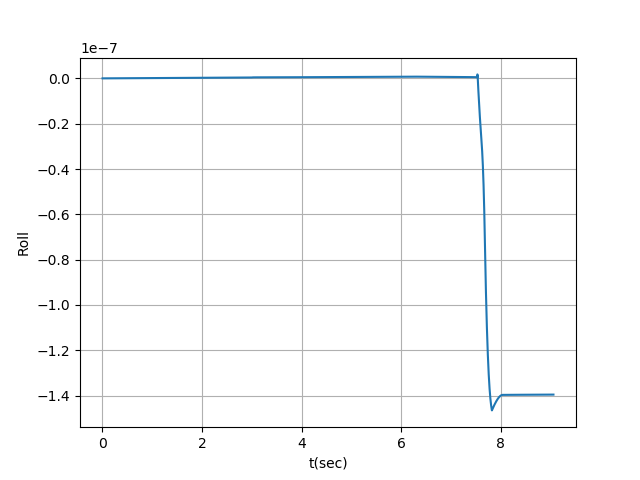
\includegraphics[width=\linewidth]{Figs/Roll.png}
                \caption{Time response of Rolling angle}
                \columnbreak

                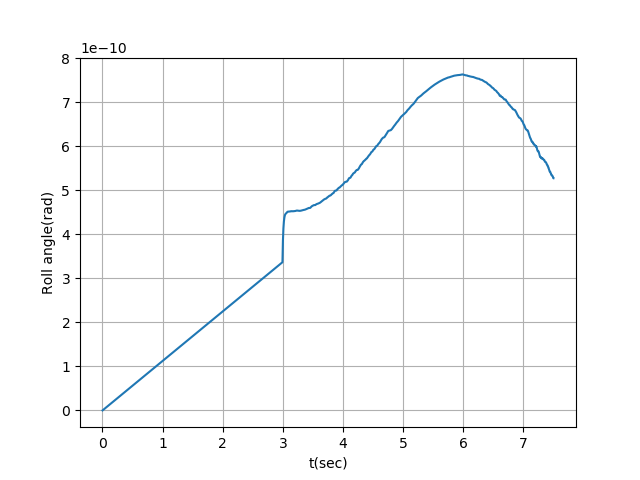
\includegraphics[width=\linewidth]{Figs/Roll_part.png}
                \caption{Time response of Roll angle until 7.5 second}
            \end{multicols}
        \end{figure}
    \end{frame}

    \begin{frame}{\secname}
        \begin{figure}
            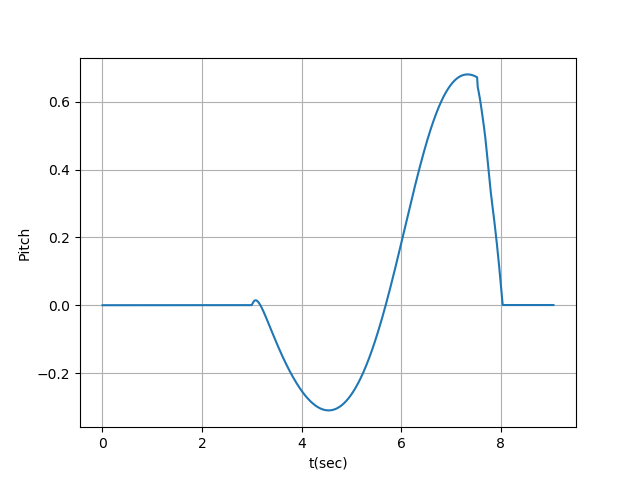
\includegraphics[width=.5\linewidth]{Figs/Pitch.png}
            \caption{Time response of Pitching angle}
        \end{figure}
    \end{frame}

    \begin{frame}{\secname}
        \begin{figure}
            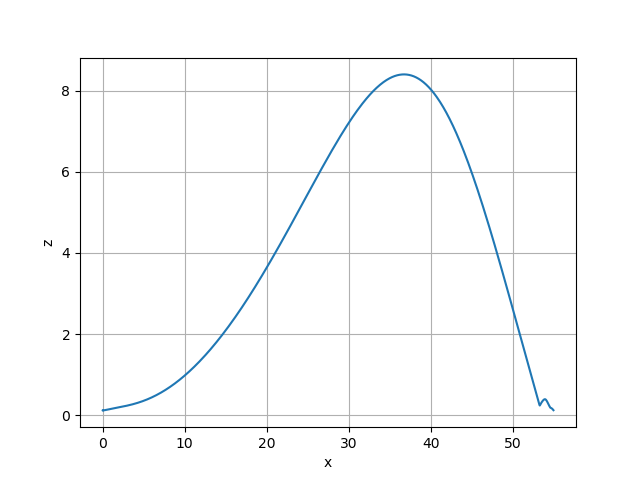
\includegraphics[width=.5\linewidth]{Figs/xz_plane.png}
            \caption{Trajectory on X-Z plane}
        \end{figure}
    \end{frame}

    \begin{frame}{\secname}
        \begin{figure}
            \begin{multicols}{2}
                \includegraphics[width=\linewidth]{Figs/x.png}
                \caption{Time response of x direction}
                \columnbreak

                \includegraphics[width=\linewidth]{Figs/z.png}
                \caption{Time response of z direction}
            \end{multicols}
        \end{figure}
    \end{frame}

\end{document}
